% \chapter{Базовые понятия и результаты}
\chapter{Обзор предметной области}
\label{ch:overview}

В данной главе представлены основные понятия и существующие результаты.


\section{Дискретные управляющие модели}
\label{sec:discrete-control-models}

Здесь описываются дискретные управляющие модели и их применение.

\subsection{Конечные автоматы}

Конечный автомат (КА) --- это модель вычислений, которая описывает систему с конечным числом состояний и переходов между ними.
Конечный автомат может быть задан в виде пятерки $\mathcal{A} = \Tuple{\Sigma, Q, q_0, F, \delta}$, где:
\begin{itemize}
    \item $\Sigma$ --- алфавит входных символов;
    \item $Q$ --- (\emph{конечное}) множество состояний;
    \item $q_0 \in Q$ --- начальное состояние;
    \item $F \subseteq Q$ --- множество терминальных (принимающих) состояний;
    \item $\delta \colon Q \times \Sigma \to Q$ --- функция переходов.
\end{itemize}
Конечный автомат \emph{принимает} (\textit{accepts}) слово $w = w_1 w_2 \ldots w_n \in \Sigma^*$, если после прочтения $w$ автомат оказывается в одном из терминальном состоянии $s_n \in F$, то есть существует последовательность состояний $s_0, s_1, \ldots, s_n$ такая, что $s_0 = q_0$, $s_{i+1} = \delta(s_i, w_{i+1})$ для всех $i \in \Set{0, 1, \ldots, n-1}$ и $s_n \in F$.

\subsection{Булевы схемы}

Булева схема --- это ациклический ориентированный граф, в котором вершины разделены на три типа: входные вершины (\textit{inputs}), выходные вершины (\textit{outputs}) и внутренние вершины (\textit{gates}).
Булева схема может быть задана в виде кортежа $\mathcal{C} = \Tuple{I, O, G, L}$, где:
\todo{пофиксить кортеж}
\begin{itemize}
    \item $I$ --- множество входных вершин (\textit{inputs});
    \item $O$ --- множество выходных вершин (\textit{outputs});
    \item $G$ --- множество внутренних вершин (\textit{gates});
% \item $W \subseteq I \union G$ --- множество входных вершин, которые не являются входами схемы (\textit{wires});
    \item $L \colon G \to \Set{\land, \lor, \neg, \dots}$ --- функция, которая каждой внутренней вершине сопоставляет логическую функцию.
\end{itemize}


\section{Задача синтеза и верификации дискретных управляющих моделей}
\label{sec:synthesis-and-verification}

...

\subsection{Синтез конечно-автоматных моделей}
\label{sub:automata-synthesis}

\subsection{Верификация конечно-автоматных моделей}
\label{sub:automata-verification}

\subsection{Синтез булевых формул и схем}
\label{sub:circuits-synthesis}

\subsection{Верификация булевых схем}
\label{sub:circuits-verification}

Задачи LEC и ATPG.

\section{Задача булевой выполнимости}
\label{sec:sat}

\subsection{Базовые определения}
\label{sub:sat-definitions}

Clause, CNF, SAT, literal, model, etc.

\subsection{Алгоритмы решения SAT}
\label{sub:sat-algorithms}

DPLL. CDCL.

\subsection{Декомпозиционная трудность}
\label{sub:sat-decomposition}

d-hardness.

\subsection{Вероятностные лазейки}
\label{sub:sat-backdoors}

Strong backdoors (or before d-hardness).
rho-backdoors.

\section{Методы сведения задач синтеза и верификации ДУ-моделей к SAT}
\label{sec:sat-encodings}


\FloatBarrier

\clearpage



% \chapter{Оформление различных элементов}
% \label{ch:ch1}

% \begin{figure}
%     \centering
%     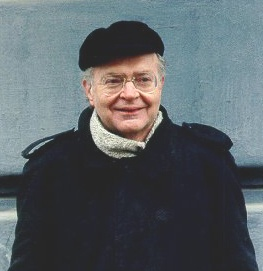
\includegraphics[width=0.6\linewidth]{images/knuth}
%     \caption{Knuth}
%     \label{fig:my_label4}
% \end{figure}


% \section{Ссылки}

% \cite{Grez2022Jul}

% \section{Форматирование чисел и размерностей величин}\label{sec:units}

% Числа форматируются при помощи команды \verb|\num|:
% \num{5,3};
% \num{2,3e8};
% \num{12345,67890};
% \num{2,6 d4};
% \num{1+-2i};
% \num{.3e45};
% \num[exponent-base=2]{5 e64};
% \num[exponent-base=2,exponent-to-prefix]{5 e64};
% \num{1.654 x 2.34 x 3.430}
% \num{1 2 x 3 / 4}.


% Обратите внимание, что ГОСТ запрещает использование знака <<->> для обозначения отрицательных чисел
% за исключением формул, таблиц и~рисунков.
% Вместо него следует использовать слово <<минус>>.

% Размерности можно записывать при помощи команд \verb|\si| и \verb|\SI|:
% \si{\farad\squared\lumen\candela};
% \si{\joule\per\mole\per\kelvin};
% \si[per-mode = symbol-or-fraction]{\joule\per\mole\per\kelvin};
% \si{\metre\per\second\squared};
% \SI{0.10(5)}{\neper};
% \SI{1.2-3i e5}{\joule\per\mole\per\kelvin};
% \SIlist{1;2;3;4}{\tesla};
% \SIrange{50}{100}{\volt}.

% \begin{table}
%     \centering
%     \captionsetup{justification=centering} % выравнивание подписи по-центру
%     \caption{Основные величины СИ}\label{tab:unit:base}
%     \begin{tabular}{llc}
%         \toprule
%         Название  & Команда                 & Символ         \\
%         \midrule
%         Ампер     & \verb|\ampere| & \si{\ampere}   \\
%         Кандела   & \verb|\candela| & \si{\candela}  \\
%         Кельвин   & \verb|\kelvin| & \si{\kelvin}   \\
%         Килограмм & \verb|\kilogram| & \si{\kilogram} \\
%         Метр      & \verb|\metre| & \si{\metre}    \\
%         Моль      & \verb|\mole| & \si{\mole}     \\
%         Секунда   & \verb|\second| & \si{\second}   \\
%         \bottomrule
%     \end{tabular}
% \end{table}

